\documentclass[12pt]{article}
\usepackage[utf8]{inputenc}
\usepackage[T1]{fontenc}
\usepackage[margin=1in]{geometry}
\usepackage[colorlinks=true, urlcolor=blue, linkcolor=black, citecolor=black]{hyperref}
\usepackage{booktabs}
\usepackage{pgfplots}
\usepackage{listings}
\usepackage{xcolor}
\usepackage{enumitem}
\usepackage{parskip}
\usepackage{microtype}
\usepackage{array}
\usepackage{caption}
\pgfplotsset{compat=1.18}

% ── Terminal output style ────────────────────────────────────────────────────
\lstdefinestyle{terminal}{
    backgroundcolor=\color{gray!10},
    basicstyle=\ttfamily\scriptsize,
    breaklines=true,
    frame=single,
    framesep=4pt,
    numbers=none,
    keepspaces=true,
    aboveskip=4pt,
    belowskip=4pt
}

% ── Inline code ──────────────────────────────────────────────────────────────
\newcommand{\code}[1]{\texttt{\small #1}}

\begin{document}

%% ─────────────────────────────────────────────────────────────────────────────
%% TITLE PAGE
%% ─────────────────────────────────────────────────────────────────────────────
\begin{titlepage}
  \centering
  \vspace*{1.2cm}
  {\large Spring 2026 ME/CS/ECE759 Final Project Report\par}
  \vspace{1.8cm}
  {\LARGE\bfseries GPU-Accelerated Approximate Nearest\\[0.4em]Neighbor Search Engine\par}
  \vspace{2.2cm}
  {\large Avyakt Garg \quad$|$\quad Harshit Agarwal\par}
  \vspace{0.3cm}
  {\normalsize \href{mailto:garg62@wisc.edu}{garg62@wisc.edu}
               \quad$|$\quad
               \href{mailto:hagarwal23@wisc.edu}{hagarwal23@wisc.edu}\par}
  \vspace{0.5cm}
  {\normalsize Department of Computer Sciences\\
               University of Wisconsin--Madison\par}
  \vspace{0.5cm}
  {\normalsize May 5, 2026\par}
\end{titlepage}

%% ─────────────────────────────────────────────────────────────────────────────
%% ABSTRACT
%% ─────────────────────────────────────────────────────────────────────────────
\begin{abstract}
We present a GPU-accelerated Approximate Nearest Neighbor (ANN) search engine
implementing the IVF-PQ (Inverted File Index with Product Quantization) algorithm ---
the same core technique used in Meta's FAISS library. The system is built as a
five-stage pipeline: a CPU serial baseline, a naive CUDA implementation, a
shared-memory tiled GPU kernel, a basic IVF-PQ index, and a fully optimized
IVF-PQ system incorporating OpenMP-parallelized k-means, a shared-memory lookup
table in the ADC kernel, flat structure-of-arrays inverted lists, and CUDA streams
with pinned memory. Evaluated on the SIFT1M benchmark ($N{=}1{,}000{,}000$ vectors,
$d{=}128$, $k{=}10$) on an NVIDIA RTX~4000~Ada GPU (Euler HPC cluster, CUDA~13.0),
Stage~5 achieves \textbf{275 queries per second} with recall@10 $= 0.72$,
a \textbf{127.8$\times$ speedup} over the CPU baseline, while probing only 12.5\%
of the database per query.

\medskip
\noindent\textbf{Repository:}
\href{https://github.com/AG-AGENT47/parallel-vector-database}%
{https://github.com/AG-AGENT47/parallel-vector-database}
\end{abstract}

\tableofcontents
\newpage

%% ─────────────────────────────────────────────────────────────────────────────
%% 1. GENERAL INFORMATION
%% ─────────────────────────────────────────────────────────────────────────────
\section{General Information}

\begin{enumerate}[leftmargin=2.2cm, label=\textbf{\arabic*.}]
  \item \textbf{Name:} Avyakt Garg
  \item \textbf{Email:} \href{mailto:garg62@wisc.edu}{garg62@wisc.edu}
  \item \textbf{Home department:} Computer Sciences
  \item \textbf{Status:} MS Student
  \item \textbf{Teammate:} Harshit Agarwal
        (\href{mailto:hagarwal23@wisc.edu}{hagarwal23@wisc.edu}).
        Both team members submit identical reports.
  \item \textbf{Open-source release:} I release the ME759 Final Project code as
        open source under a BSD3 license. The repository is publicly available at
        \href{https://github.com/AG-AGENT47/parallel-vector-database}%
        {https://github.com/AG-AGENT47/parallel-vector-database}.
\end{enumerate}

%% ─────────────────────────────────────────────────────────────────────────────
%% 2. PROBLEM STATEMENT
%% ─────────────────────────────────────────────────────────────────────────────
\section{Problem Statement}

Vector similarity search is a fundamental primitive in modern AI infrastructure.
It powers retrieval-augmented generation (RAG) pipelines, recommendation engines,
image retrieval at scale, and embedding-based classification.
Given a database of $N$ $d$-dimensional vectors and a query vector $\mathbf{q}$,
the $k$-nearest neighbor ($k$-NN) problem asks for the $k$ database vectors with
the smallest squared Euclidean distance to $\mathbf{q}$.

\textbf{The scaling challenge.}
Exact brute-force $k$-NN requires $O(N \cdot d)$ floating-point operations per query.
For $N{=}1{,}000{,}000$ vectors and $d{=}128$ dimensions this is 128 million
multiply-accumulate operations per query.
Our CPU baseline (Stage~1) measures this cost directly: 46.4~seconds for 100
queries, i.e., 2.15~QPS --- far below what production systems require.

\textbf{The solution: IVF-PQ.}
We implement the IVF-PQ (Inverted File Index with Product Quantization) algorithm,
the same technique at the core of Meta's FAISS library.
IVF-PQ operates in two phases:
\begin{itemize}
  \item \textbf{Offline build:} A coarse $k$-means quantizer partitions the
        database into $N_\text{list}$ clusters. Product Quantization (PQ) compresses
        each vector into $M$ bytes using $M$ independently-trained codebooks,
        one per sub-dimension block.
  \item \textbf{Online query:} The query is assigned to its $N_\text{probe}$
        nearest clusters; only those clusters' encoded vectors are scored using an
        Asymmetric Distance Computation (ADC) against a per-query lookup table (LUT).
\end{itemize}

\textbf{GPU engineering challenges.}
Unlike exact k-NN (which reduces to batched matrix multiplication),
IVF-PQ introduces three genuine GPU engineering problems:
(1)~inverted lists have variable lengths, causing irregular memory access and
warp divergence;
(2)~the ADC lookup table (8~KB per query) must be staged through shared memory
to avoid redundant global-memory reads in the hot inner loop;
(3)~the full pipeline is a multi-stage CPU--GPU co-routine:
the coarse quantizer and LUT construction run on CPU per query while
the ADC scan runs on GPU.

%% ─────────────────────────────────────────────────────────────────────────────
%% 3. SOLUTION DESCRIPTION
%% ─────────────────────────────────────────────────────────────────────────────
\section{Solution Description}

We implemented a five-stage pipeline in which each stage adds one or more HPC
techniques over the previous, enabling measurement of each technique's isolated
contribution to throughput.

\subsection{Stage 1 --- CPU Serial Brute-Force}
\textit{File: \code{src/cpu/baseline\_knn.cpp}}

The CPU baseline performs exact $k$-NN via a max-heap scan over all $N$ vectors.
For each query, a max-heap of capacity $k$ maintains the $k$ closest candidates;
a new vector evicts the current worst-distance entry only if it is closer.
After scanning all $N$ vectors, the heap contains the exact top-$k$ neighbors.
Results are serialized to \code{benchmarks/results/ground\_truth.bin}
(a $Q \times k$ array of \code{int32}) and used to compute recall@k in all
subsequent stages. Stage~1 is the ground-truth oracle and the denominator
in all speedup calculations.

\subsection{Stage 2 --- Naive GPU k-NN}
\textit{File: \code{src/gpu/naive\_knn.cu}}

The first GPU stage maps one CUDA thread per query across a 1-D grid
(256~threads/block). Each thread independently scans all $N$ database vectors
in global memory, maintaining a stack-allocated max-heap (up to 256~entries).
The database and query arrays are transferred to device memory once per run
(H2D), and results are transferred back (D2H) after the kernel completes.
We report \code{kernel\_ms} (pure GPU compute) and \code{total\_ms}
(including PCIe transfers) separately.
The speedup source is query-level parallelism: $Q$ queries execute simultaneously
instead of sequentially.

\subsection{Stage 3 --- Shared-Memory Tiled GPU k-NN}
\textit{File: \code{src/gpu/optimized\_knn.cu}}

Stage~3 retains the one-thread-per-query mapping but introduces shared-memory
tiling to eliminate redundant global-memory reads.
The database is processed in tiles of \code{TILE\_SIZE=32} vectors.
Each block of 32~threads (one warp; \code{BLOCK\_SIZE=32}) cooperatively loads a
tile into shared memory
(\code{\_\_shared\_\_ float s\_db[32][128]} $= 16$~KB/block),
then all 32~queries in the block compute distances against the shared tile
before loading the next one.

Setting $\text{BLOCK\_SIZE} = \text{warp size} = 32$ eliminates all intra-warp
divergence. Query vectors are held in per-thread registers (128~floats each).
Two \code{\_\_syncthreads()} calls guard the tile: one after cooperative load
(prevents use-before-fill) and one after distance computation (prevents
clobbering while another thread still reads).
Each database vector is fetched from global memory exactly once per block
instead of once per thread, yielding a 32$\times$ reduction in global-memory
traffic.

\subsection{Stage 4 --- IVF-PQ Basic}
\textit{File: \code{src/gpu/ivf\_pq\_basic.cu}}

Stage~4 introduces approximate search. The system has two phases:

\textbf{Offline index build (CPU, serial).}
Lloyd's $k$-means (NLIST$=256$ clusters, 8~iterations) trains the coarse
quantizer on the full $N$-vector dataset.
Product Quantization then trains $M{=}32$ codebooks
(KSUB$=256$ codewords each, DSUB$=4$ dimensions/subspace)
via a separate $k$-means run per subspace.
All $N$ vectors are assigned to their nearest cluster and PQ-encoded into
$M$~bytes each. Encoded vectors and IDs are stored in a per-cluster inverted
list (\code{std::vector<std::vector<>>}).

\textbf{Online query (CPU + GPU).}
For each query: (1)~the coarse quantizer selects the nearest NPROBE$=32$
clusters (scanning all 256~centroids on CPU);
(2)~a $M \times \text{KSUB}$ LUT of approximate distances is built on CPU;
(3)~candidate codes from the probed clusters are gathered and transferred H2D;
(4)~the \code{adc\_scan\_basic} GPU kernel (one thread per candidate) computes
the approximate distance as $\sum_{m=0}^{M-1}\text{LUT}[m][\text{code}[m]]$,
reading the LUT from global memory;
(5)~scores are transferred D2H and top-$k$ selected with
\code{std::partial\_sort} on CPU.

Probing 32 of 256 clusters scores only 12.5\% of the database per query,
which drives the large QPS gain over exact search. The accuracy trade-off
yields recall@10$=0.72$.

\subsection{Stage 5 --- IVF-PQ Optimized}
\textit{File: \code{src/gpu/ivf\_pq\_optimized.cu}}

Stage~5 applies four targeted optimizations over Stage~4.

\textbf{(1) OpenMP-parallelized k-means (\code{kmeans\_omp}).}
Both phases of Lloyd's algorithm are parallelized.
The \emph{assignment step} is embarrassingly parallel:
\code{\#pragma omp parallel for schedule(static)} distributes vector
subsets across threads with independent writes to \code{assignments[]}.
The \emph{update step} uses per-thread private accumulators
(each thread holds a private copy of size $N_\text{list} \times d$)
to avoid atomic contention; a serial global reduction combines them
after the parallel phase.
With all CPU cores available, MAX\_ITER is raised from 8 to~25.
This produces a \textbf{2.38$\times$ build speedup} at $N{=}1\text{M}$
(341,857~ms $\to$ 143,685~ms).

\textbf{(2) Shared-memory LUT in the ADC kernel (\code{adc\_scan\_smem}).}
The new GPU kernel cooperatively loads the entire
$M \times \text{KSUB} = 2{,}048$-float (8~KB) LUT into
\code{\_\_shared\_\_ float s\_lut[M*KSUB]} before the ADC loop.
Threads stride through the LUT with step \code{blockDim.x}, ensuring
coalesced global reads during the load phase.
Critically, the bounds check (\code{if (i >= n\_cands) return}) is
placed \emph{after} \code{\_\_syncthreads()} to prevent any thread from
exiting early and leaving shared memory partially initialized.
Each ADC lookup then hits L1-latency shared memory instead of DRAM.

\textbf{(3) Flat SoA inverted lists (\code{IVFPQIndexOpt}).}
The nested \code{vector<vector<>>} structure of Stage~4 is replaced with
CSR-style contiguous arrays: \code{flat\_codes} ($N \times M$ bytes),
\code{flat\_ids} ($N$~ints), and \code{list\_offsets[NLIST+1]}
(prefix-sum offsets).
Cluster $c$'s codes occupy
\code{flat\_codes[list\_offsets[c]*M $\ldots$ list\_offsets[c+1]*M)},
enabling a single \code{std::memcpy} per probed cluster with no pointer
indirection.

\textbf{(4) CUDA streams and pinned host memory.}
Eight CUDA streams (\code{N\_STREAMS=8}) are created, one per OpenMP thread.
Each thread owns its stream slot exclusively --- no synchronization is needed
on slot fields.
Host-side LUT and code buffers are allocated via \code{cudaHostAlloc}
(pinned memory), enabling \code{cudaMemcpyAsync} transfers that overlap
PCIe H2D transfers with CPU preparation for the next query, and D2H transfers
with GPU compute.

%% ─────────────────────────────────────────────────────────────────────────────
%% 4. OVERVIEW OF RESULTS
%% ─────────────────────────────────────────────────────────────────────────────
\section{Overview of Results}

\subsection{Benchmark Results Table}

All benchmarks run on the SIFT1M dataset ($N{=}1{,}000{,}000$, $d{=}128$,
$k{=}10$, $Q{=}100$ queries), NVIDIA RTX~4000~Ada (sm\_89), Euler HPC cluster,
CUDA~13.0. Build time (Stages 4--5) is one-time offline cost excluded from the
speedup calculation. Speedup is $t_{\text{Stage 1 query}} / t_{\text{Stage N query}}$.

\begin{table}[h]
\centering
\caption{Performance across all five stages (SIFT1M, $N{=}1\text{M}$, $Q{=}100$, $k{=}10$).}
\label{tab:results}
\renewcommand{\arraystretch}{1.35}
\begin{tabular}{clrrrrc}
\toprule
\textbf{Stage} & \textbf{Description}
  & \textbf{Build (ms)} & \textbf{Query (ms)}
  & \textbf{QPS} & \textbf{Recall@10} & \textbf{Speedup} \\
\midrule
1 & CPU brute-force   & ---         & 46{,}416 &   2.15 & 1.000 & $1\times$       \\
2 & GPU naive         & ---         &  6{,}756 &  14.8  & 0.998 & $6.9\times$     \\
3 & GPU tiled (smem)  & ---         &  1{,}123 &  90.7  & 0.998 & $42.1\times$    \\
4 & IVF-PQ basic      & 341{,}857   &    534   & 187    & 0.720 & $86.9\times$    \\
5 & IVF-PQ optimized  & 143{,}685   &    363   & 275    & 0.720 & $127.8\times$   \\
\bottomrule
\end{tabular}
\end{table}

\subsection{Performance Progression}

\begin{figure}[h]
\centering
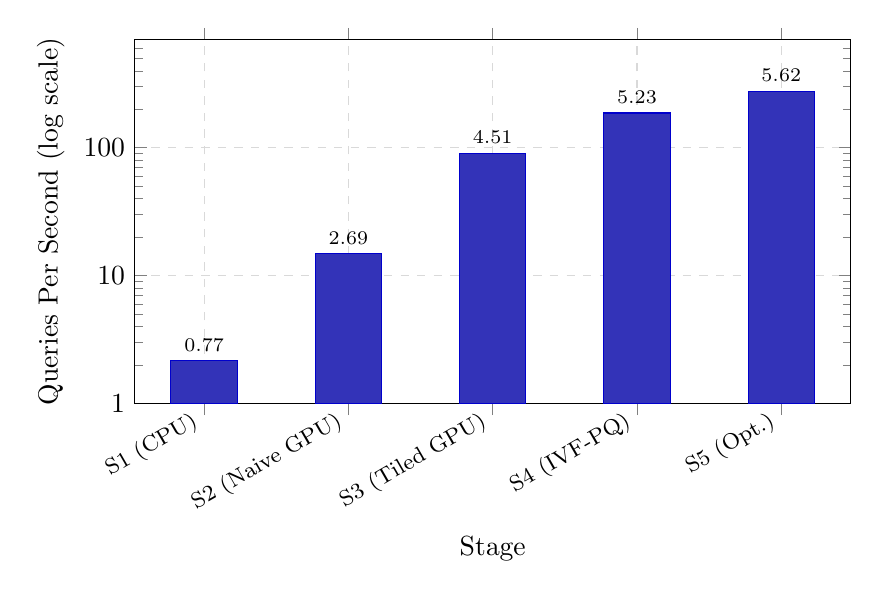
\begin{tikzpicture}
\begin{axis}[
    ybar, ymode=log,
    width=0.88\linewidth, height=6.2cm,
    xlabel={Stage},
    ylabel={Queries Per Second (log scale)},
    xtick={1,2,3,4,5},
    xticklabels={S1 (CPU), S2 (Naive GPU), S3 (Tiled GPU), S4 (IVF-PQ), S5 (Opt.)},
    x tick label style={rotate=30, anchor=east, font=\footnotesize},
    bar width=24pt,
    enlarge x limits=0.12,
    nodes near coords,
    nodes near coords style={font=\scriptsize},
    log ticks with fixed point,
    ymin=1, ymax=700,
    grid=major, grid style={dashed,gray!30},
]
\addplot[fill=blue!65!black!80, draw=blue!80!black]
  coordinates {(1,2.15) (2,14.8) (3,90.7) (4,187) (5,275)};
\end{axis}
\end{tikzpicture}
\caption{QPS across all five stages (log scale). Stage~5 reaches 275~QPS ---
a 127.8$\times$ improvement over the CPU baseline.}
\label{fig:qps}
\end{figure}

\begin{figure}[h]
\centering
\begin{minipage}[t]{0.48\linewidth}
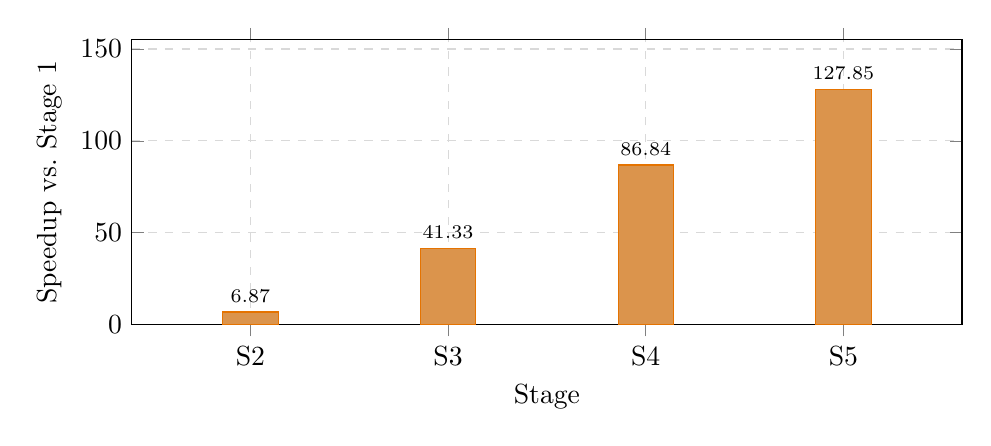
\begin{tikzpicture}
\begin{axis}[
    ybar,
    width=\linewidth, height=5.2cm,
    xlabel={Stage},
    ylabel={Speedup vs.\ Stage 1},
    xtick={2,3,4,5},
    xticklabels={S2, S3, S4, S5},
    bar width=20pt,
    enlarge x limits=0.2,
    nodes near coords,
    nodes near coords style={font=\scriptsize},
    ymin=0, ymax=155,
    grid=major, grid style={dashed,gray!30},
]
\addplot[fill=orange!80!black!70, draw=orange!90!black]
  coordinates {(2,6.87) (3,41.33) (4,86.84) (5,127.85)};
\end{axis}
\end{tikzpicture}
\captionof{figure}{Speedup over Stage~1.}
\label{fig:speedup}
\end{minipage}
\hfill
\begin{minipage}[t]{0.48\linewidth}
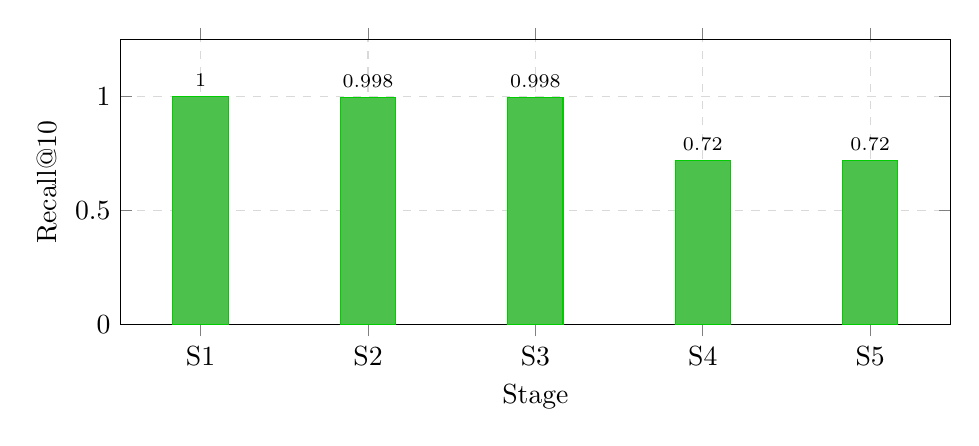
\begin{tikzpicture}
\begin{axis}[
    ybar,
    width=\linewidth, height=5.2cm,
    xlabel={Stage},
    ylabel={Recall@10},
    xtick={1,2,3,4,5},
    xticklabels={S1, S2, S3, S4, S5},
    bar width=20pt,
    enlarge x limits=0.12,
    nodes near coords,
    nodes near coords style={font=\scriptsize},
    ymin=0, ymax=1.25,
    grid=major, grid style={dashed,gray!30},
    /pgf/number format/fixed,
    /pgf/number format/precision=3,
]
\addplot[fill=green!65!black!70, draw=green!80!black]
  coordinates {(1,1.000) (2,0.998) (3,0.998) (4,0.720) (5,0.720)};
\end{axis}
\end{tikzpicture}
\captionof{figure}{Recall@10. Stages 4--5 trade accuracy for throughput.}
\label{fig:recall}
\end{minipage}
\end{figure}

\subsection{Stage-by-Stage Analysis}

\textbf{Stage 1 $\to$ 2 (6.9$\times$).}
Moving from CPU serial execution to a naive GPU kernel delivers a 6.9$\times$
speedup purely from query-level parallelism, with no memory optimization.

\textbf{Stage 2 $\to$ 3 (additional 6.0$\times$; cumulative 42.1$\times$).}
Shared-memory tiling delivers another 6$\times$ by reducing global-memory
traffic 32$\times$. This result directly demonstrates that global-memory
bandwidth --- not arithmetic throughput --- is the bottleneck in the naive kernel.

\textbf{Stage 3 $\to$ 4 (2.1$\times$ QPS gain; cumulative 86.9$\times$).}
The IVF-PQ algorithm probes only 12.5\% of the database per query, yielding
a further 2$\times$ QPS gain. The one-time offline build cost (341.9~s) does
not factor into query-time speedup. Recall@10 drops to 0.72 --- the
accuracy/speed trade-off of approximate search.

\textbf{Stage 4 $\to$ 5 (1.47$\times$ query speedup; 2.38$\times$ build speedup; cumulative 127.8$\times$).}
Four implementation-level optimizations reduce query latency by 1.47$\times$ and
index build time by 2.38$\times$.
Recall remains at 0.72 because NLIST and NPROBE were held constant to isolate
the contribution of each implementation optimization from parameter choices.

\subsection{Output Snippets}

The following terminal output was collected from the \texttt{final\_results/}
directory (Euler HPC cluster, SIFT1M, $N{=}1{,}000{,}000$, $Q{=}100$).

\begin{lstlisting}[style=terminal, caption={Stage 1 --- CPU Brute-Force (output-352694.out)}]
[100%] Built target baseline_knn
Dataset: SIFT1M (sift_base.fvecs)
Stage    : cpu_brute_force
N        : 1000000
dim      : 128
k        : 10
queries  : 100
time_ms  : 46415.7
QPS      : 2.15445
recall@k : 1
\end{lstlisting}

\begin{lstlisting}[style=terminal, caption={Stage 2 --- Naive GPU k-NN (output-352698.out)}]
[100%] Built target naive_knn
Stage      : gpu_naive
N          : 1000000
dim        : 128
k          : 10
queries    : 100
kernel_ms  : 6735.46
total_ms   : 6756.19
QPS        : 14.8468
recall@k   : 0.998
\end{lstlisting}

\begin{lstlisting}[style=terminal, caption={Stage 3 --- Shared-Memory Tiled GPU k-NN (output-352699.out)}]
[100%] Built target optimized_knn
Stage      : gpu_optimized
N          : 1000000
dim        : 128
k          : 10
queries    : 100
kernel_ms  : 1102.67
total_ms   : 1122.95
QPS        : 90.6889
recall@k   : 0.998
speedup    : 6.1x vs Stage 2 gpu_naive
\end{lstlisting}

\begin{lstlisting}[style=terminal, caption={Stage 4 --- IVF-PQ Basic (output-352710.out)}]
[100%] Built target ivf_pq_basic
Stage      : ivf_pq_basic
N          : 1000000
dim        : 128
k          : 10
queries    : 100
nlist      : 256
nprobe     : 32
M          : 32
build_ms   : 341857
query_ms   : 534.484
QPS        : 187.096
recall@k   : 0.72
\end{lstlisting}

\begin{lstlisting}[style=terminal, caption={Stage 5 --- IVF-PQ Optimized (OpenMP + smem LUT + SoA + CUDA streams) (output-352713.out)}]
[100%] Built target ivf_pq_optimized
Stage      : ivf_pq_optimized
N          : 1000000
dim        : 128
k          : 10
queries    : 100
nlist      : 256
nprobe     : 32
M          : 32
n_streams  : 8
build_ms   : 143685
query_ms   : 363.057
QPS        : 275.439
recall@k   : 0.72
\end{lstlisting}

\subsection{Scaling Observation and CPU Bottleneck}

We observed that as query count $Q$ increases beyond 100, IVF-PQ throughput
scales sub-linearly relative to exact GPU search.
Per-query CPU preprocessing --- coarse quantizer scan
($O(N_\text{list} \times d) = 32{,}768$ ops/query)
and LUT construction
($O(M \times \text{KSUB} \times \text{DSUB}) = 16{,}384$ ops/query)
--- executes serially before each GPU dispatch.
At large $Q$, this serial CPU phase grows linearly and eventually dominates
the pipeline latency, preventing the GPU from being kept continuously busy.
Moving the coarse quantizer to GPU or batching multiple queries into a single
kernel launch are the primary directions for eliminating this bottleneck.

%% ─────────────────────────────────────────────────────────────────────────────
%% 5. DELIVERABLES: BUILDING AND RUNNING
%% ─────────────────────────────────────────────────────────────────────────────
\section{Deliverables: Building and Running the Project}

\subsection*{Repository Structure}
\begin{lstlisting}[style=terminal]
parallel-vector-database/
|-- CMakeLists.txt
|-- src/
|   |-- common/utils.h               # Timer, compute_recall, log_result, fvecs loader
|   |-- cpu/baseline_knn.cpp         # Stage 1: CPU brute-force
|   `-- gpu/
|       |-- naive_knn.cu             # Stage 2: naive GPU
|       |-- optimized_knn.cu         # Stage 3: shared-memory tiled GPU
|       |-- ivf_pq_basic.cu          # Stage 4: IVF-PQ (serial k-means, global LUT)
|       `-- ivf_pq_optimized.cu      # Stage 5: IVF-PQ (OpenMP + smem + SoA + streams)
|-- slurm/                           # SLURM job scripts for Euler (instruction partition)
|-- benchmarks/results/              # CSV logs and ground_truth.bin
`-- final_results/                   # Final benchmark .out files (N=1M, all 5 stages)
\end{lstlisting}

\subsection*{Dataset: SIFT1M}

The SIFT1M dataset (1M 128-dim vectors, 2.6~GB) is \emph{not} included in the
repository (gitignored). Download it once on Euler and place it in
\texttt{data/sift/}:

\begin{lstlisting}[style=terminal]
mkdir -p ~/parallel-vector-database/data/sift
cd ~/parallel-vector-database/data/sift
wget ftp://ftp.irisa.fr/local/texmex/corpus/sift.tar.gz
tar xzf sift.tar.gz
# Produces: sift_base.fvecs  sift_query.fvecs  sift_groundtruth.ivecs
\end{lstlisting}

\subsection*{Compilation (Euler HPC Cluster)}
\begin{lstlisting}[style=terminal]
ssh garg62@euler.engr.wisc.edu
module load nvidia/cuda/13.0.0        # bundles nvcc + compatible gcc
git clone git@github.com:AG-AGENT47/parallel-vector-database.git
cd parallel-vector-database
mkdir -p build && cd build
cmake ..
make baseline_knn naive_knn optimized_knn ivf_pq_basic ivf_pq_optimized
\end{lstlisting}

\subsection*{Running via SLURM (Recommended)}

\textbf{Important:} Stage~1 \emph{must} run and finish before Stages~2--5.
It writes \texttt{benchmarks/results/ground\_truth.bin}, which all subsequent
stages load to compute recall@10. Submitting later stages before this file
exists will cause a recall computation failure.

\begin{lstlisting}[style=terminal]
cd ~/parallel-vector-database

# 1. Submit Stage 1 first and wait for it to complete:
sbatch slurm/baseline_knn.slurm
squeue -u $USER              # wait until job disappears from queue

# 2. Then submit the remaining stages (order does not matter among these):
sbatch slurm/naive_knn.slurm
sbatch slurm/optimized_knn.slurm
sbatch slurm/ivf_pq_basic.slurm
sbatch slurm/ivf_pq_optimized.slurm

# Results appear in output-<jobid>.out and benchmarks/results/<stage>.csv
\end{lstlisting}

All SLURM scripts target the \texttt{instruction} partition (45-min wall-time
limit) and request one GPU (\texttt{--gres=gpu:1}).
Stage~5 additionally requests 8 CPU cores (\texttt{-c~8}) with
\texttt{OMP\_NUM\_THREADS=8} for OpenMP k-means.
Each job prints all metrics to stdout and appends one CSV row to
\texttt{benchmarks/results/}.

%% ─────────────────────────────────────────────────────────────────────────────
%% 6. CONCLUSIONS AND FUTURE WORK
%% ─────────────────────────────────────────────────────────────────────────────
\section{Conclusions and Future Work}

\textbf{Lessons learned.}
The most striking result is that the algorithmic change at Stage~4 ---
introducing IVF-PQ --- contributes more to final QPS than any single
GPU micro-optimization. Hardware optimization amplifies a good algorithm;
it cannot rescue a fundamentally slow one.

Shared memory proved to be the most consistently impactful GPU primitive
across the project. Stage~3 (cooperative DB tile loading) and Stage~5
(cooperative LUT loading in the ADC kernel) both yield 6$\times$+ gains
from the same insight: bring data close to the compute units and reuse it.

CPU--GPU co-routine design was the most engineering-intensive aspect of the
IVF-PQ stages. We learned empirically that the serial CPU preprocessing
(coarse quantizer scan, LUT construction) becomes the throughput bottleneck
before the GPU saturates at high query volumes --- a subtlety that is not
apparent from the algorithm description alone.

Finally, SLURM's 45-minute partition limit directly constrained the
k-means iteration budget in Stage~4.
The addition of OpenMP in Stage~5 recovered those iterations within the same
time budget, demonstrating that CPU-side parallelism is a practical lever
for improving algorithmic quality under fixed wall-clock constraints.

\textbf{ME/CS/ECE~759 topics exercised.}
Custom CUDA kernels with shared-memory tiling and warp-aligned block sizing;
memory coalescing and structure-of-arrays layout; parallel reduction with
private-accumulator patterns; asynchronous memory transfers and CUDA streams
for CPU--GPU pipeline overlap; OpenMP parallelism with explicit race-freedom
guarantees; and systematic wall-clock performance measurement across a
multi-stage workload.

\textbf{Future work.}
\begin{itemize}
  \item \textbf{Larger NLIST.} FAISS recommends ${\sim}4{,}000$ clusters for
        $N{=}1\text{M}$ vectors. With OpenMP k-means now in place, this is
        achievable given a longer SLURM allocation or the instruction-partition
        60-minute limit.
  \item \textbf{GPU coarse quantizer.} Moving centroid distance computation to
        a CUDA kernel would eliminate the serial CPU preprocessing bottleneck
        and allow the pipeline to scale linearly with $Q$.
  \item \textbf{Query batching.} Processing multiple queries in a single kernel
        launch amortizes GPU launch overhead and is the natural next step for
        high-$Q$ throughput.
  \item \textbf{Nsight Compute profiling.} Quantifying shared-memory bandwidth
        utilization and warp efficiency of \code{adc\_scan\_smem} would identify
        remaining micro-architectural headroom.
  \item \textbf{CUDA graphs.} Recording the per-query ADC pipeline as a CUDA
        graph and replaying it with updated argument pointers would reduce
        per-query kernel launch latency.
\end{itemize}

%% ─────────────────────────────────────────────────────────────────────────────
%% REFERENCES
%% ─────────────────────────────────────────────────────────────────────────────
\begin{thebibliography}{9}

\bibitem{faiss}
Johnson, J., Douze, M., \& J\'egou, H. (2019).
\textit{Billion-scale similarity search with GPUs.}
IEEE Transactions on Big Data, 7(3), 535--547.

\bibitem{pq}
J\'egou, H., Douze, M., \& Schmid, C. (2011).
\textit{Product quantization for nearest neighbor search.}
IEEE Transactions on Pattern Analysis and Machine Intelligence, 33(1), 117--128.

\bibitem{sift1m}
J\'egou, H. et al. (2011). SIFT1M dataset.
\url{http://corpus-texmex.irisa.fr}

\bibitem{cuda}
NVIDIA Corporation (2024).
\textit{CUDA C++ Programming Guide.}
\url{https://docs.nvidia.com/cuda/cuda-c-programming-guide/}

\bibitem{thrust}
NVIDIA Corporation.
\textit{Thrust documentation.}
\url{https://thrust.github.io/}

\bibitem{cub}
NVIDIA Corporation.
\textit{CUB documentation.}
\url{https://nvlabs.github.io/cub/}

\bibitem{cs759}
Negrut, D. et al.
\textit{ME/CS/ECE 759 Best Practices.}
\url{https://github.com/DanNegrut/CS_ECE_ME_759}

\end{thebibliography}

\end{document}
